
\typeout{new file: Validation_Tests_Chapter.tex}

\chapter{Validation Tests}
\label{chap::validation_tests}

This chapter presents some validations tests that have been performed with the latest version of RadCal. The first six cases presented in this chapter are from the previous Grosshandler report~\cite{Grosshandler1993}. For these tests, the numbering is similar to that of the aforementioned reference. In each test, predictions from the latest version of RadCal are compared with those obtained with the former version of RadCal. Test 1 compares values of {$\rm CO_2$} total emissivity at fixed temperature as function of pressure path-length. Test 2 compares values of {$\rm CO_2$} total emissivity at fixed pressure path-length as function of temperature. Test 3 compares values of {$\rm H_2O$} total emissivity at fixed temperature as function of pressure path-length. Test 4 compares values of {$\rm H_2O$} total emissivity at fixed pressure path-length as function of temperature. Test 5 compares the spectral intensity and transmittance profiles obtained from the simulation of a simplified pool fire. Test 6 compares the spectral transmittance and spectral incident radiance from a methane rich premixed flame. Test 7 is a new test included in this report. It simulates the spectral transmissivity and incident spectral intensity to the surface of a methanol 30~cm diameter pool fire. Experimental temperature and species mole fraction data were obtained experimentally by Aykut Yilmaz and were published in Ref.~\cite{Yilmaz2008}.


\section{Test 1: isothermal {$\rm CO_2$}}

This test compares estimates of {$\rm CO_2$} of intensity and transmissivity obtained with the previous and latest version of RADCAL as a function of pressure-path length, $P_iL$. The original version of RadCal is referred to as ``Old RadCal'' and the latest version as ``New RadCal''. This test also compares at selected values the total emissivity as defined by Eq.~\ref{eq:total_emissivity} from the New RadCal with those published in the previous RadCal report~\cite{Grosshandler1993}. These values are referred to as ``TN1402''. Values extracted from the Hottel chart and presented in Ref.~\cite{Grosshandler1993} are also reported under ``Hottel''.
Figure~\ref{fig:Test1_CO2_Hottel} plots the estimates from the New RadCal as a function of pressure path-length in the top figure. The bottom figure plots the integrated relative error in intensity, denoted $\epsilon_{rad}$, and transmissivity, denoted $\epsilon_{\tau}$, between the two versions of RadCal as a function of pressure path-length. Values are given in percent. The relative error on transmissivity $\epsilon_{\tau}$ was calculated as:

\begin{equation}\label{eq:epsilon_tau}
 \epsilon_{\tau} = \displaystyle\int_{50}^{10000} \displaystyle\frac{|\tau_{Old\,RadCal}-\tau_{Old\,RadCal}|}{\tau_{Old\,RadCal}}{\d \om}.
\end{equation}
Similar expression was applied to compute $\epsilon_{rad}$. The total pressure was set to 1.0~atm, the temperature to 1500~K and $\rm CO_2$ mole fraction to $5.0 \times 10^{-3}$. Air was mixed with ${\rm CO_2}$. The total pressure and the amount of ${\rm CO_2}$ were kept constant. The length of the homogeneous cell was varied to cover the desired range.

\begin{figure}
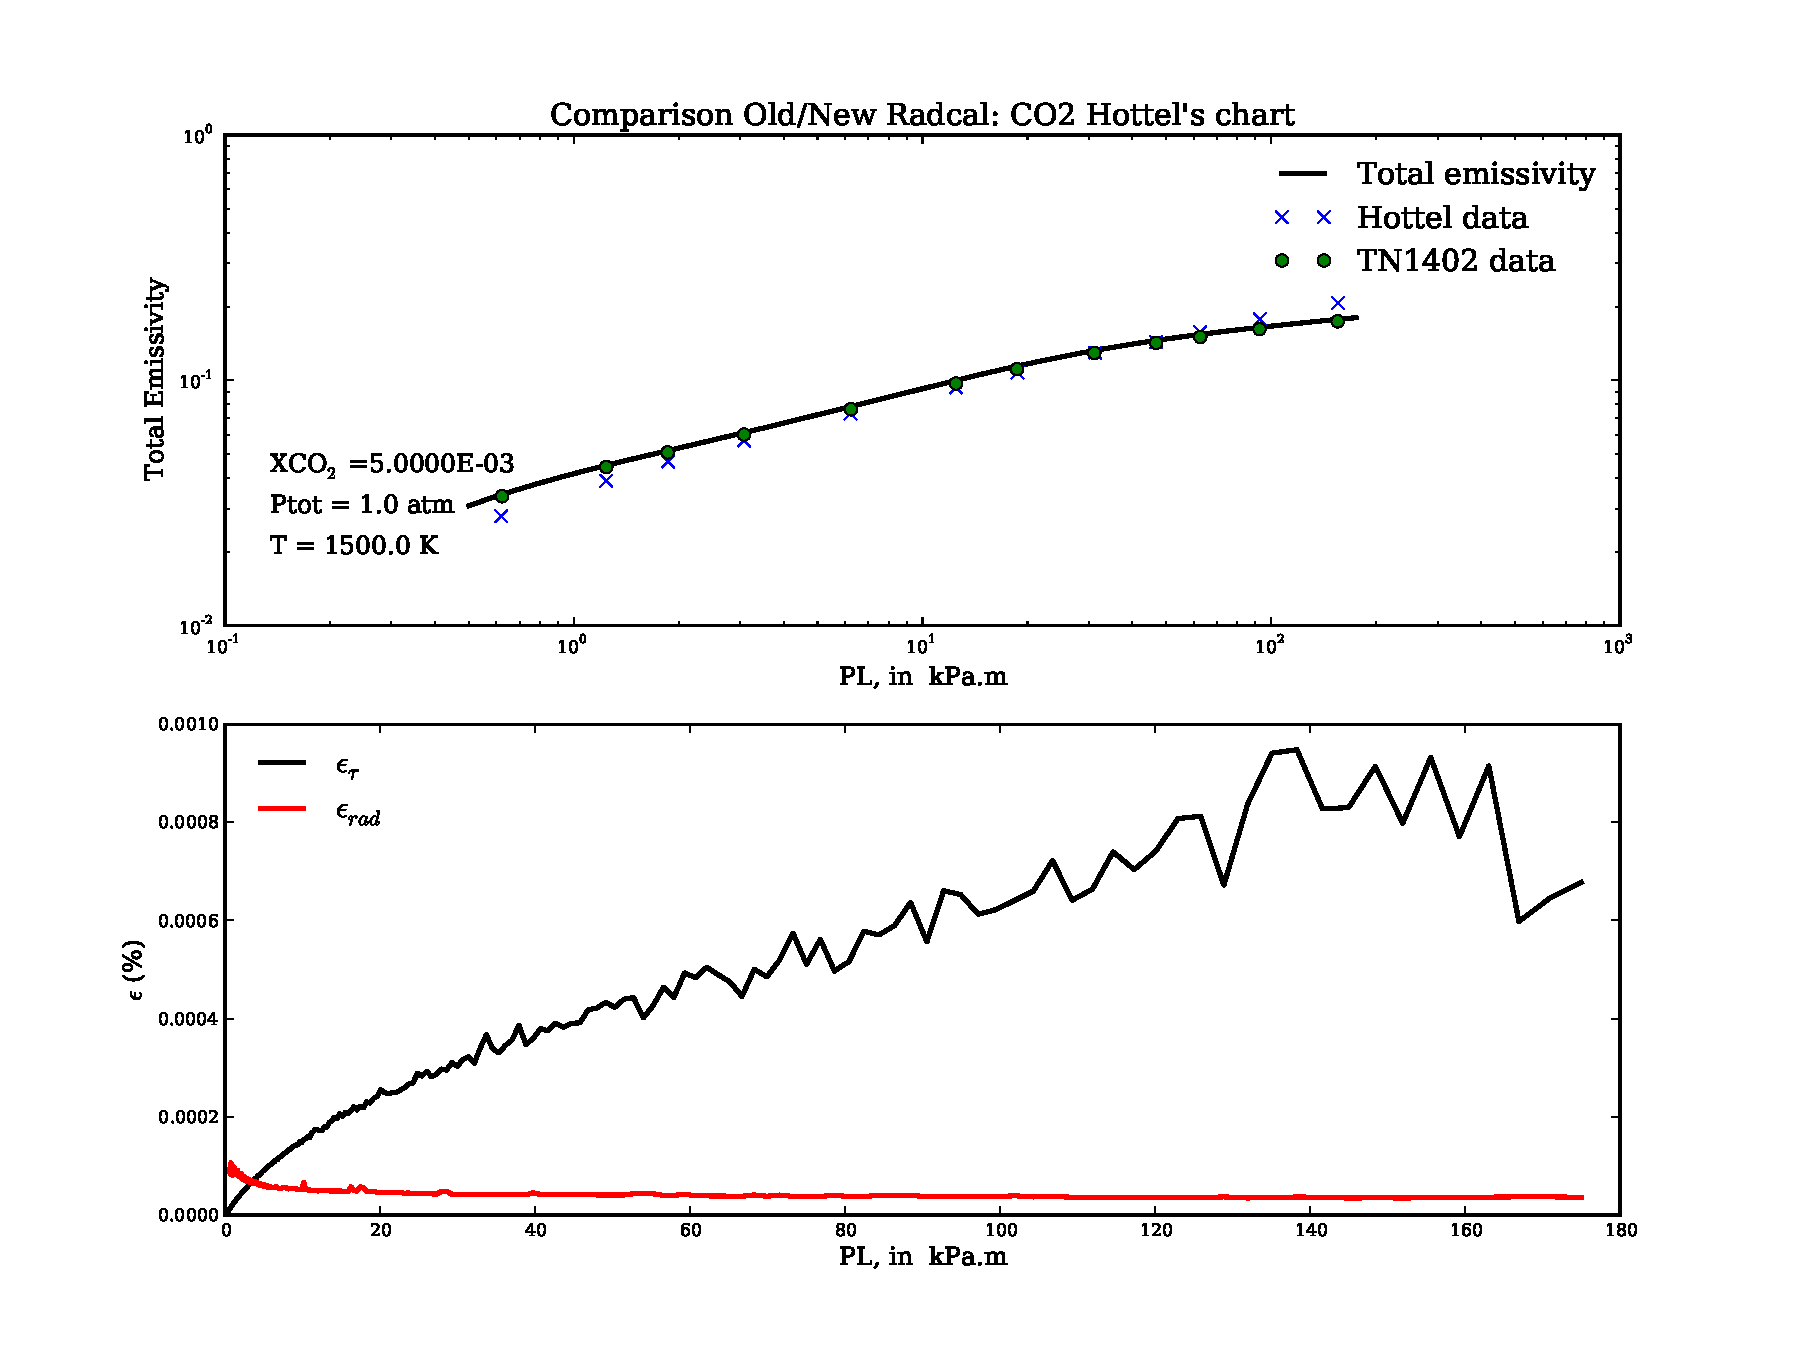
\includegraphics[width=\textwidth]{Figures/Test1_CO2_Hottel.pdf}.
\caption{Top: total emissivity, as defined by Eq.~\ref{eq:total_emissivity}, of isothermal, homogeneous ${\rm CO_2}$/air mixtures as a function of the pressure path-length. Temperature was set at 1500~K, the mole fraction of ${\rm CO_2}$ was set at $5.0\times10^{-3}$ and the total pressure is set at 1~atm. Solid line indicates estimates obtained with the latest version of RadCal, the crossed symbols indicate Hottel data, and the filled circles are data extracted from Grosshandler~\cite{Grosshandler1993}.
Bottom: integrated relative error between the old RadCal and the new RadCal in spectral transmissivity, denoted $\epsilon_{\tau}$, and spectral intensity, denoted $\epsilon_{rad}$, as defined by Eq.~\ref{eq:epsilon_tau}. Values are given in percentage.\label{fig:Test1_CO2_Hottel}}
\end{figure}

The agreement between the two versions of RadCal for the simulations of a isothermal, homogeneous layer of ${\rm CO_2}$, is very good. The new version of RadCal does not change the results of ${\rm CO_2}$ simulations, which it should not as the $\rm CO_2$ data have not been modified from the previous version.



\section{Test 2: fixed pressure path-length {$\rm CO_2$ }}

This second test compares the predictions of the two RadCal versions with the data from Hottel. In this test, $\rm CO_2$ is mixed with air. The total pressure is  set to 1~atm, and the mole fraction of $\rm CO_2$ is set to $5 \times 10^{-3}$. The physical length is set to 36~m. The medium is assumed homogeneous and isothermal. The temperature of the mixture is varied between 300~K to 2800~K. Similarly to Test~1, the total emissivity as defined by Eq.~\ref{eq:total_emissivity} is reported on the top Fig.~\ref{fig:Test2_CO2_Hottel} and the integrated relative error between the old RadCal and the new RadCal in spectral transmissivity, denoted $\epsilon_{\tau}$, and spectral intensity, denoted $\epsilon_{rad}$, as defined by Eq.~\ref{eq:epsilon_tau}, are reported on the bottom Fig.~\ref{fig:Test2_CO2_Hottel}.

Overall very good agreement is obtained between the two RadCals and between RadCal and the Hottel data. Some discrepancies are observed between Hottel data and the RadCal predictions at low (around 300~K) and high temperatures (above 2000~K).
A small discrepancy (<2 \%) exists between the old and new versions of RadCal in the temperature range 1200-1500~K. This small discrepancy is attributed to a slightly better interpolation at this temperature range for the $\rm CO_2$ Band 1 (between 500 -- 800~cm$^{-1}$).

\begin{figure}
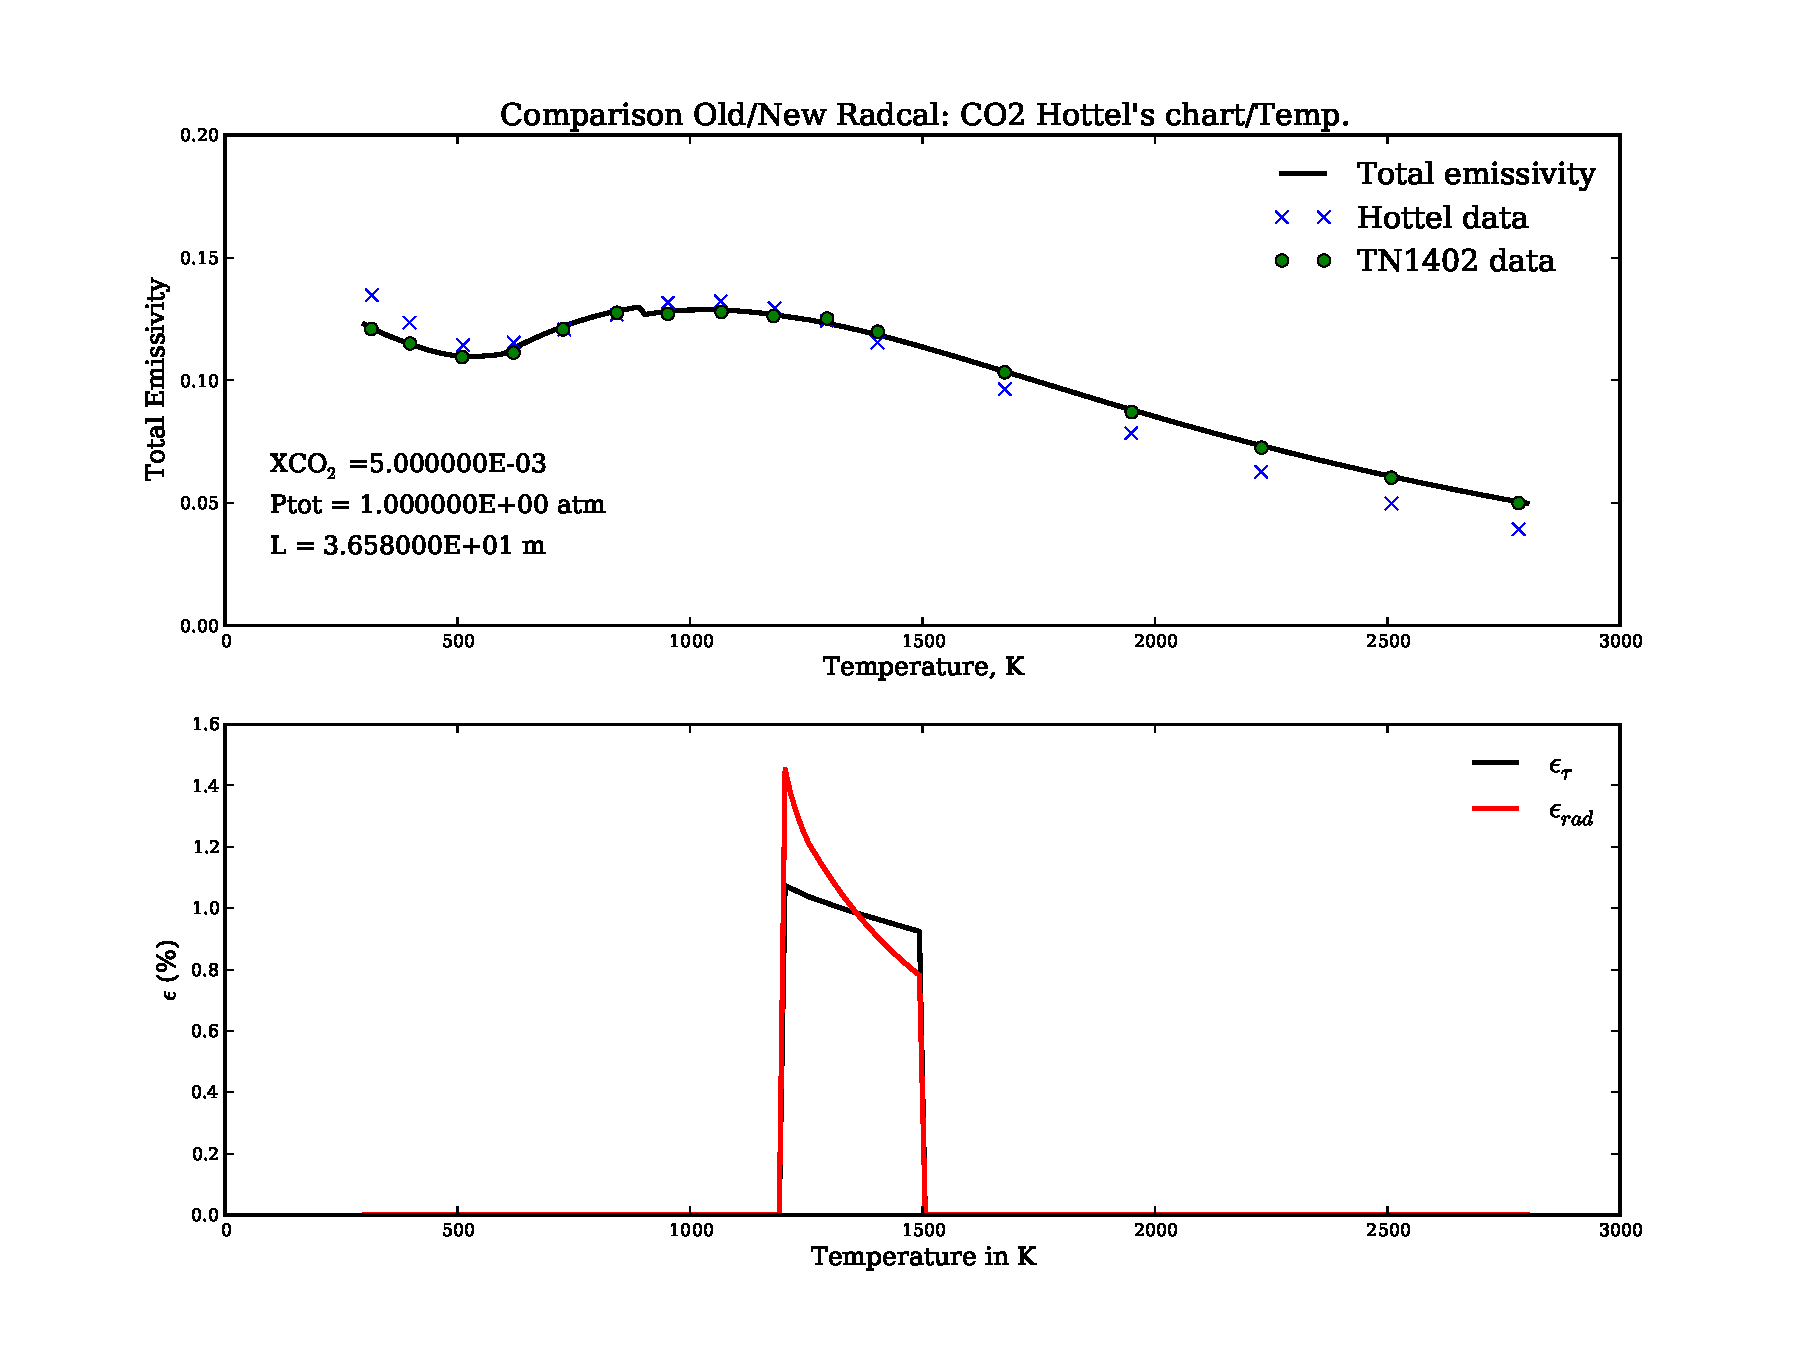
\includegraphics[width=\textwidth]{Figures/Test2_CO2_Hottel.pdf}
\caption{Top: total emissivity, as defined by Eq.~\ref{eq:total_emissivity}, of homogeneous ${\rm CO_2}$/air mixtures as a function of the mixture temperature. The mole fraction of ${\rm CO_2}$ was set at $5.0 \times 10^{-3}$, and the total pressure is set at 1~atm. Solid line indicates estimates obtained with the latest version of RadCal, crossed symbols are Hottel data, and filled circles are data extracted from Grosshandler~\cite{Grosshandler1993}. Bottom: integrated relative error between the old RadCal and the new RadCal in spectral intensity, denoted $\epsilon_{\tau}$, and spectral intensity, denoted $\epsilon_{rad}$. Values are given in percentage.\label{fig:Test2_CO2_Hottel}}
\end{figure}


\section{Test 3: isothermal {$\rm H2O$ }}

This test is almost identical to Test 1, the only difference lies in the choice of $\rm H_2O$ as the participating species. The configuration is that of a homogeneous column of $\rm H_2O$ mixed with air set at a pressure of 1~atm. The mole fraction of $\rm H_2O$ is set at $5 \times 10^{-3}$ and the temperature is 1500~K. The physical length of the domain was varied between 1~m to 300~m.

This test compares at selected values the predicted total emissivity as defined by Eq.~\ref{eq:total_emissivity} from the New RadCal with those published in the previous RadCal report~\cite{Grosshandler1993}. Results are plotted in Fig.~\ref{fig:Test3_H2O_Hottel}. These values are referred to as ``TN1402''. Values extracted from the Hottel chart and presented in Ref.~\cite{Grosshandler1993} are also reported under ``Hottel''. This test also compares the predicted values of the spectral intensity and transmissivity from the two RadCal versions. Very good agreement is obtained between the two versions of RadCal, and good agreement between the Hottel and RadCal data is obtained. It is noteworthy that this new version of RadCal does change the predictions when using $\rm H_2O$.

\begin{figure}
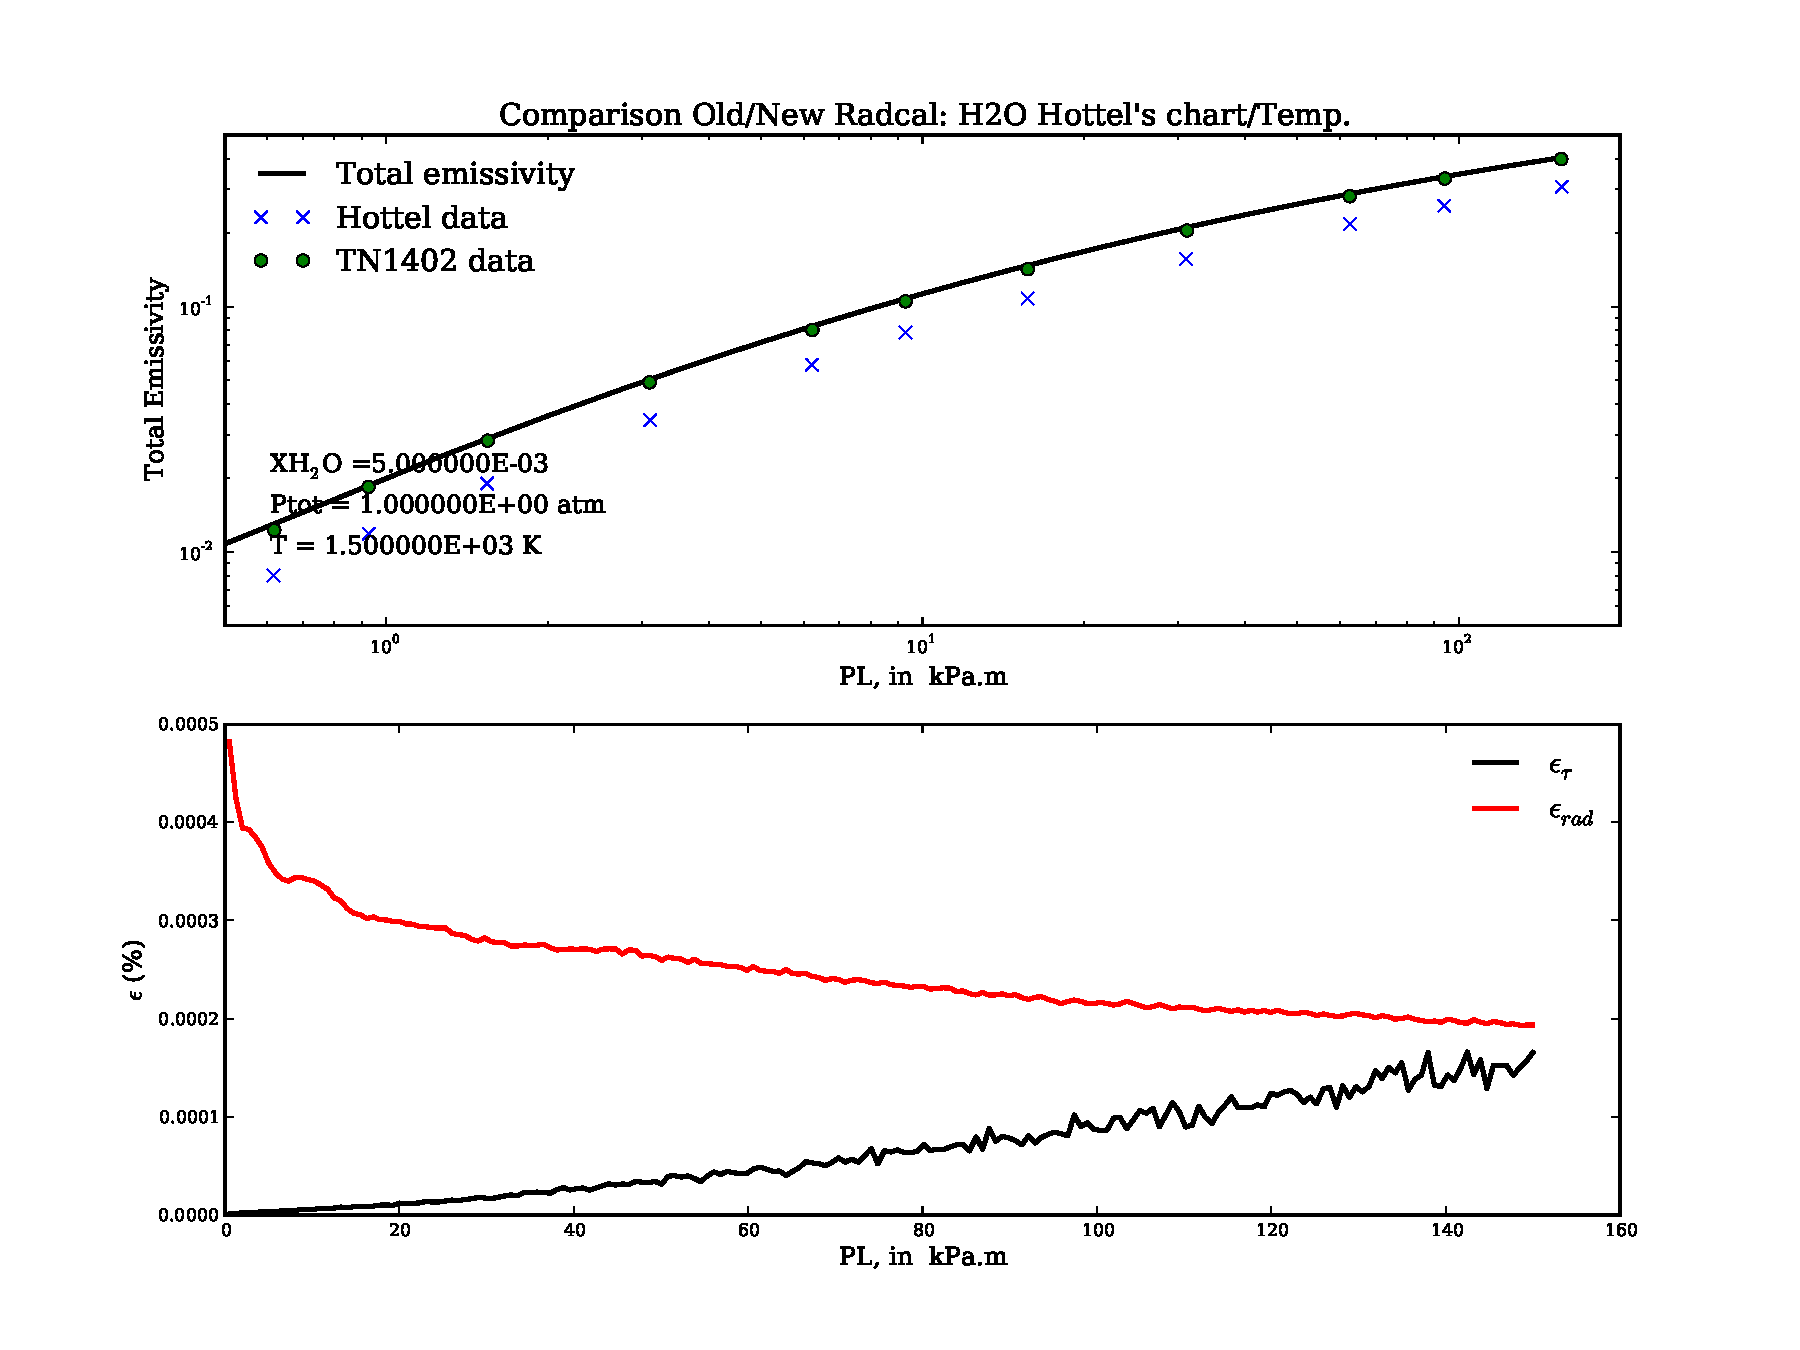
\includegraphics[width=\textwidth]{Figures/Test3_H2O_Hottel.pdf}
\caption{Top: total emissivity, as defined by Eq.~\ref{eq:total_emissivity}, of isothermal, homogeneous ${\rm H_2O}$/air mixtures as a function of the pressure path-length. Temperature was set at 1500~K, the mole fraction of ${\rm H_2O}$ was set at $5.0 \times 10^{-3}$, and the total pressure is set at 1~atm. Solid line indicates estimates obtained with the latest version of RadCal, crossed symbols are Hottel data, and filled circles are data extracted from Grosshandler~\cite{Grosshandler1993}. Bottom: integrated relative error between the old RadCal and the new RadCal in spectral intensity, denoted $\epsilon_{\tau}$, and spectral intensity, denoted $\epsilon_{rad}$. Values are given in percentage.\label{fig:Test3_H2O_Hottel}}
\end{figure}


\section{Test 4: fixed pressure path-length {$\rm H_2O$}}

This fourth test is very similar to Test~2, excepts that $\rm H_2O$ is used as participating species. Variations of the total emissivity of a homogeneous column of a $\rm H_2O$-air mixture of 30.48~m length with the mixture temperature is plotted in Fig.~\ref{fig:Test4_H2O_Hottel} and compared with the previous data of Hottel and the previous RadCal prediction, referred to here as ``TN1402'', as reported in Grosshandler~\cite{Grosshandler1993}. Temperature is varied between 200~K and 2600~K. Evolution of the total emissivity as defined by Eq.~\ref{eq:total_emissivity} with temperature is reported in Fig.~\ref{fig:Test4_H2O_Hottel}. Overall good agreement is reproduced between the old version of RadCal and the new one except near ambient temperature where some discrepancies exist. There are due to a small spurious spike that is present in the previous version of RadCal in the spectral range 500 -- 800~cm$^{-1}$ which is not physical. This spurious spike disappears above 300~K. The new version of RadCal does not feature this spike. Similar discrepancies as those reported in Grosshandler~\cite{Grosshandler1993} remain between Hottel data and RadCal in the total emissivity of $\rm H_2O$, as plotted in Fig.~\ref{fig:Test4_H2O_Hottel}. As Grosshandler wrote in Ref.~\cite{Grosshandler1993}: \textit{``...Ludwig~\cite{Ludwig1973} pointed out that the earlier work by Hottel covered a more limited range of conditions and attempted to minimize the number of parameters for engineering estimates, and, thus, should not be expected to be as accurate as the narrow-band calculations.''}

\begin{figure}
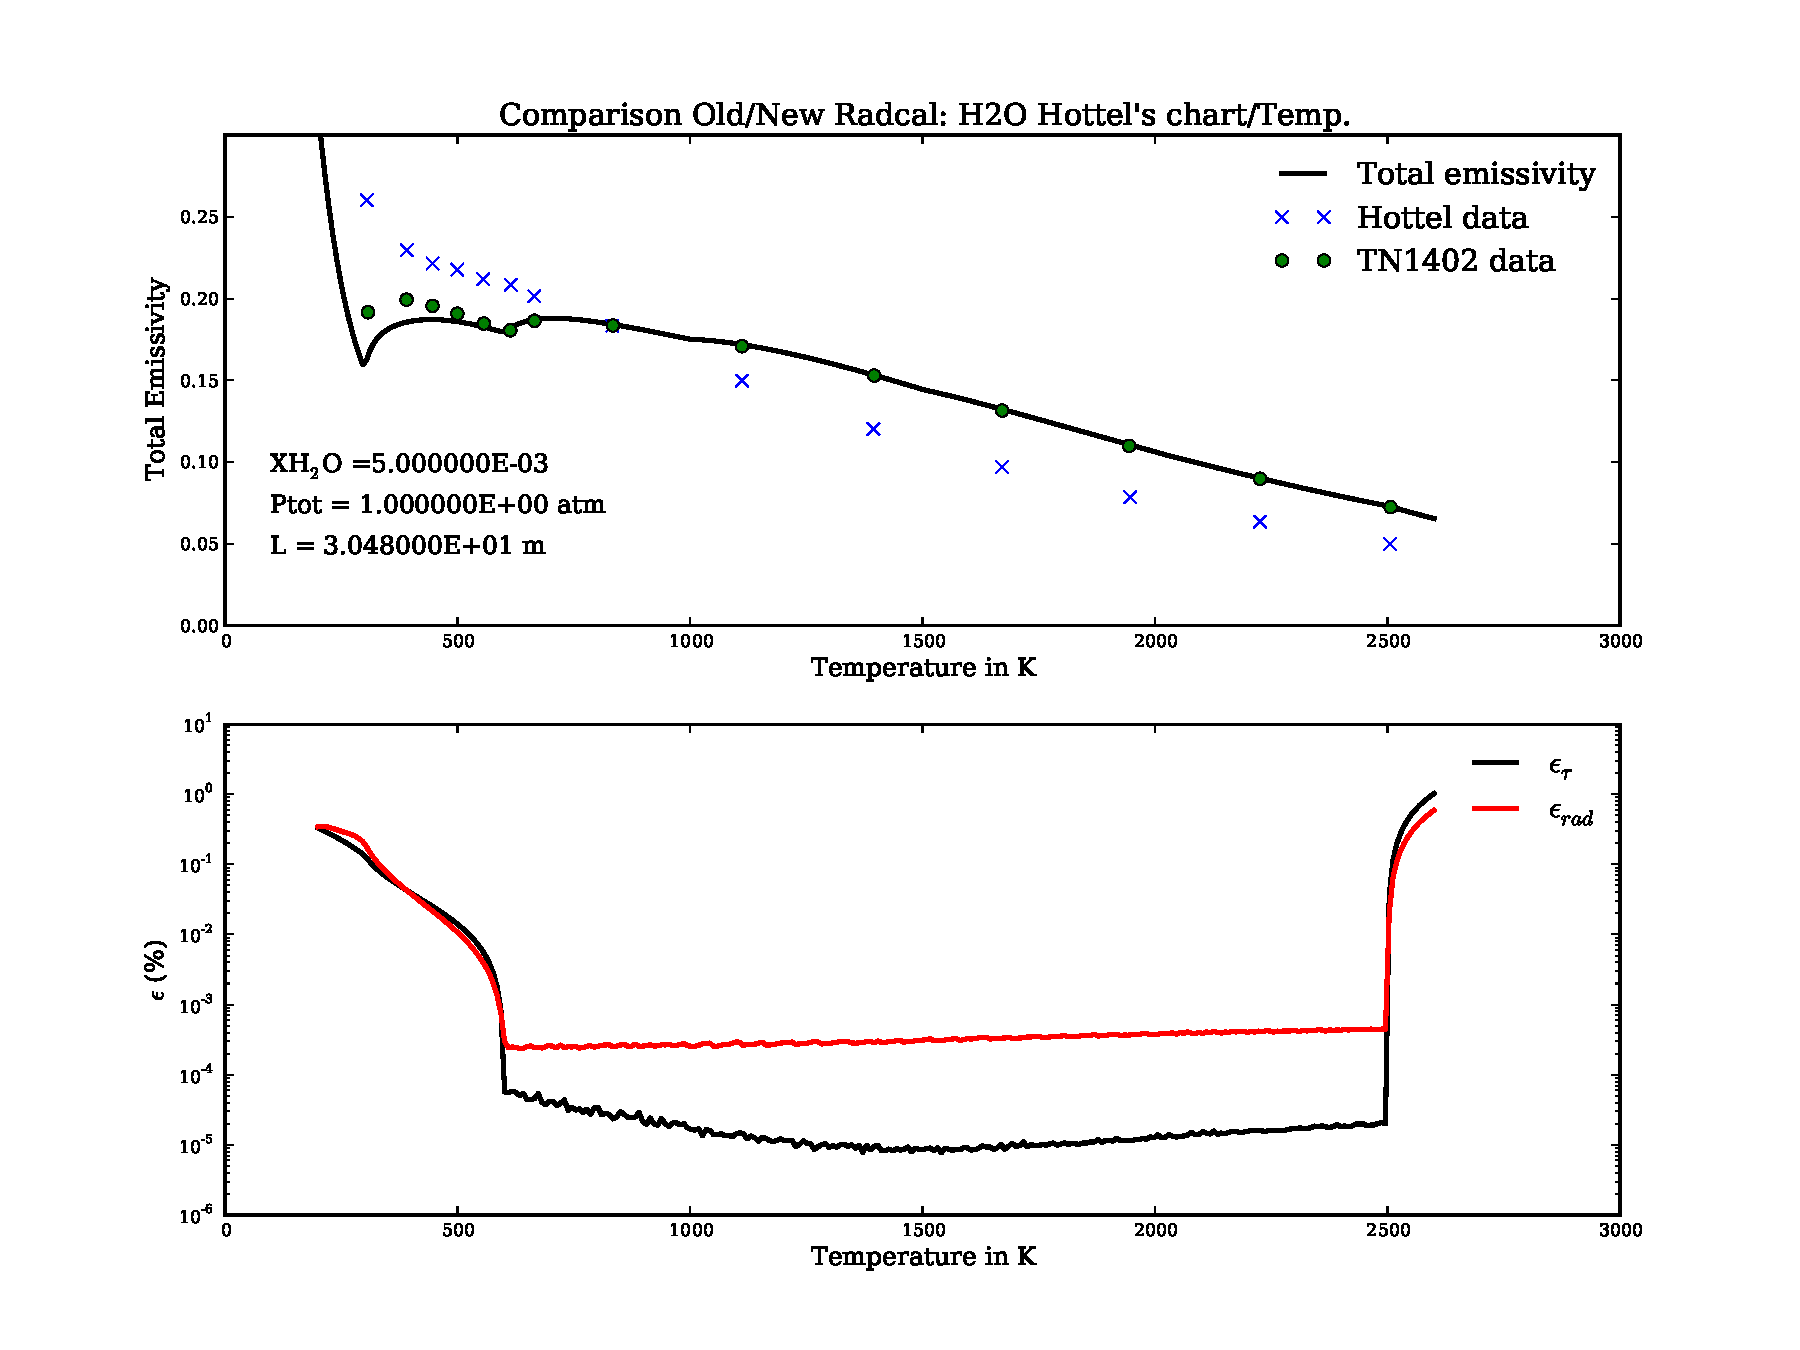
\includegraphics[width=\textwidth]{Figures/Test4_H2O_Hottel.pdf}
\caption{Top: total emissivity, as defined by Eq.~\ref{eq:total_emissivity}, of homogeneous ${\rm H_2O}$/air mixtures as a function of the temperature. The physical length is set to 30.48~m, the mole fraction of ${\rm H_2O}$ was set at $5.0 \times 10^{-3}$ and the total pressure is set at 1~atm. The temperature was varied between 200 to 2800~K. Solid line indicates estimates obtained with the latest version of RadCal, crossed symbols are Hottel data, and filled circles are data extracted from Grosshandler~\cite{Grosshandler1993}. Bottom: integrated relative error between the old RadCal and the new RadCal in spectral intensity, denoted $\epsilon_{\tau}$, and spectral intensity, denoted $\epsilon_{rad}$. Values are given in percentage.\label{fig:Test4_H2O_Hottel}}
\end{figure}


\section{Test 5: simulated one meter diameter pool fire}

This test compares the predictions from the old and new versions of RadCal from a simulated one meter diameter fire that contains $\rm CO_2$, $\rm H_2O$, and soot. Table~\ref{table::test5_fire} gives the temperature, species, and soot concentration as a function of the distance from the observer. Figure~\ref{fig:Test5_Poolfire} plots the predicted spectral transmissivity (top) and the predicted spectral incident intensity from the old version of RadCal (given in red) and the new version of RadCal (given in black). Excellent agreement between the two versions is obtained. Table~\ref{table::received_flux} reports the predicted received total intensities from the old and the new versions of RadCal. Excellent agreement is obtained between the two versions.

\begin{table}[ht]
      \centering
\caption{Radial profile through simulated one meter diameter pool fire.\label{table::test5_fire}}
\begin{tabular}{|c|c|c|c|c|c|} \hline
Distance (cm) & Temperature (K) & X$_{CO2}$ & X$_{H2O}$ & X$_{N2}$ & f$_v$  \\
\hline
5  & 899  & 0.070 & 0.070 & 0.860 & $5.55\times 10^{-8}$\\
10 & 1158 & 0.099 & 0.099 & 0.802 & $5.55\times 10^{-8}$\\
20 & 1438 & 0.130 & 0.130 & 0.741 & $5.55\times 10^{-8}$\\
30 & 1637 & 0.152 & 0.152 & 0.695 & $5.55\times 10^{-8}$\\
50 & 1770 & 0.167 & 0.167 & 0.665 & $5.55\times 10^{-8}$\\
70 & 1637 & 0.152 & 0.152 & 0.695 & $5.55\times 10^{-8}$\\
80 & 1438 & 0.130 & 0.130 & 0.741 & $5.55\times 10^{-8}$\\
90 & 1158 & 0.099 & 0.099 & 0.802 & $5.55\times 10^{-8}$\\
95 & 899  & 0.070 & 0.070 & 0.860 & $5.55\times 10^{-8}$\\
\hline
\end{tabular}
\end{table}

\begin{table}
\centering
\caption{Predicted received intensity from the old and the new versions of RadCal for the simulated one meter diameter pool fire described in Table~\ref{table::test5_fire}.\label{table::received_flux}}
\begin{tabular}{|c|c|c|} \hline
 Quantity & Old Radcal &New RadCal \\
\hline
 Received total intensity (W/m$^{-2}$/str) & 33784.3 & 33746.9\\
\hline
\end{tabular}
\end{table}

\begin{figure}
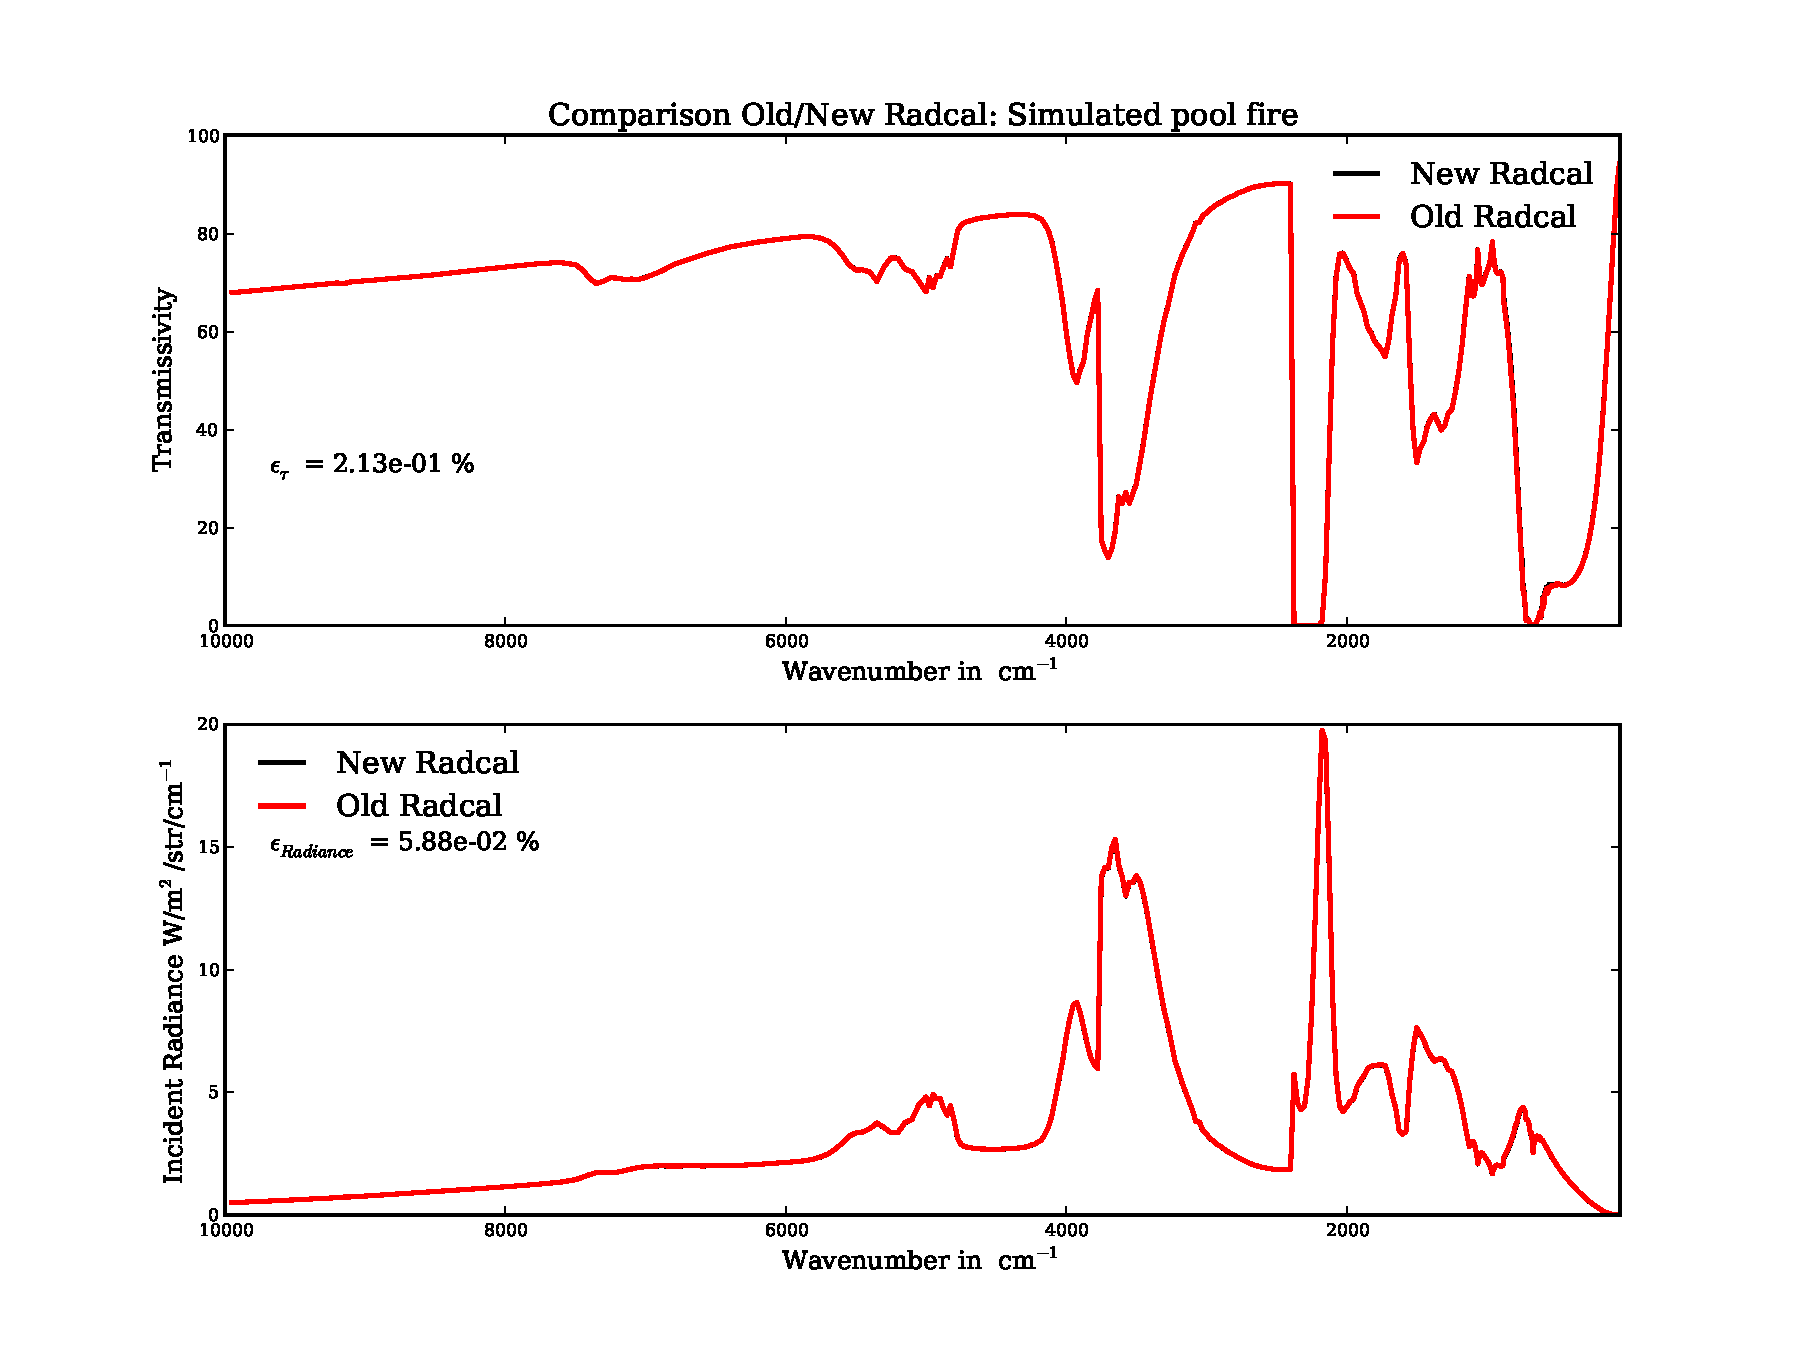
\includegraphics[width=\textwidth]{Figures/Comp_old_new_Pool_fire.pdf}
\caption{Top: Spectral transmissivity, $\bar{\tau}(\om_0; 1000 \rightarrow 0)$, in \%, for a simulated one meter diameter pool fire. Red line: predicted results using the previous version of RadCal. Black line: predicted profile using the new version of RadCal. Bottom: predicted incident spectral intensity, $I_{\om_0}(0)$, given in $\rm W/m^{2}/str/cm^{-1}$ .\label{fig:Test5_Poolfire}}
\end{figure}


\section{Test 6: methane premixed flame}

Figure~\ref{fig:Test6_Premixed} represents the predicted spectral transmissivity and  spectral incident intensity by the old and the new versions of RadCal for a 20~mm thick fuel rich premixed methane/$\rm N_2$/$\rm O_2$ flame at 606~kPa. Predictions with the new RadCal version were performed using the newest $\rm CH_4$ data. The input file for the new version is given below:
\begin{lstlisting}
&HEADER TITLE="Figure6_New_Radcal" CHID="Figure6_New_Radcal" /

&BAND
	OMMIN = 50.0
	OMMAX = 10000.0 /
&WALL TWALL = 0.0 /

&Path_Segment ! Define a homogeneous segment
	T        = 300.0    ! Temperature in Kelvin
	LENGTH   = 0.002    ! Length of the segment in meters
	PRESSURE = 6.0      ! Pressure in atm
	XCO2     = 0.0000E+000   ! Mole fraction of CO2
	XH2O     = 0.0000E+000   ! Mole fraction of H2O
        XCH4     = 2.0165E-001   ! Mole fraction of CH4
        XCO      = 0.0000E+000   ! Mole fraction of CO
        XO2      = 3.0660E-001   ! Mole fraction of O2
	XN2      = 4.9175E-001 / ! Mole fraction of N2

&Path_Segment ! Define a homogeneous segment
	T        = 725.0         ! Temperature in Kelvin
	LENGTH   = 0.0020        ! Length of the segment in meters
	PRESSURE = 6.0000E+000   ! Pressure in atm
	XCO2     = 0.0000E+000   ! Mole fraction of CO2
	XH2O     = 9.6700E-002   ! Mole fraction of H2O
        XCH4     = 1.5330E-001   ! Mole fraction of CH4
        XCO      = 4.8350E-002   ! Mole fraction of CO
        XO2      = 2.3003E-001   ! Mole fraction of O2
	XN2      = 4.7162E-001 / ! Mole fraction of N2

&Path_Segment ! Define a homogeneous segment
	T        = 1150.0        ! Temperature in Kelvin
	LENGTH   = 0.0020        ! Length of the segment in meters
	PRESSURE = 6.0554E+000   ! Pressure in atm
	XCO2     = 0.0000E+000   ! Mole fraction of CO2
	XH2O     = 1.9163E-001   ! Mole fraction of H2O
        XCH4     = 1.0235E-001   ! Mole fraction of CH4
        XCO      = 9.7450E-002   ! Mole fraction of CO
        XO2      = 1.5942E-001   ! Mole fraction of O2
	XN2      = 4.4915E-001 / ! Mole fraction of N2

&Path_Segment ! Define a homogeneous segment
	T        = 1575.0        ! Temperature in Kelvin
	LENGTH   = 0.0020        ! Length of the segment in meters
	PRESSURE = 6.1901E+000   ! Pressure in atm
	XCO2     = 0.0000E+000   ! Mole fraction of CO2
	XH2O     = 2.9079E-001   ! Mole fraction of H2O
        XCH4     = 5.0065E-002   ! Mole fraction of CH4
        XCO      = 1.5675E-001   ! Mole fraction of CO
        XO2      = 7.9175E-002   ! Mole fraction of O2
	XN2      = 4.2322E-001 / ! Mole fraction of N2

&Path_Segment ! Define a homogeneous segment
	T        = 2000.0       ! Temperature in Kelvin
	LENGTH   = 0.0040        ! Length of the segment in meters
	PRESSURE = 6.1198E+000   ! Pressure in atm
	XCO2     = 8.0890E-003   ! Mole fraction of CO2
	XH2O     = 3.6272E-001   ! Mole fraction of H2O
        XCH4     = 1.6350E-002   ! Mole fraction of CH4
        XCO      = 1.7327E-001   ! Mole fraction of CO
        XO2      = 2.4591E-002   ! Mole fraction of O2
	XN2      = 4.1498E-001 / ! Mole fraction of N2

&Path_Segment ! Define a homogeneous segment
	T        = 2525.0        ! Temperature in Kelvin
	LENGTH   = 0.0055        ! Length of the segment in meters
	PRESSURE = 6.1495E+000   ! Pressure in atm
	XCO2     = 8.0400E-003   ! Mole fraction of CO2
	XH2O     = 3.9350E-001   ! Mole fraction of H2O
        XCH4     = 0.0000E+000   ! Mole fraction of CH4
        XCO      = 1.8870E-001   ! Mole fraction of CO
        XO2      = 0.0000E+000   ! Mole fraction of O2
	XN2      = 4.0976E-001 / ! Mole fraction of N2
#--------------------------------------------------------------------------------
\end{lstlisting}
Very good agreement between the two versions is obtained. The main difference lies in the $\rm C-H$ stretch band of methane (2700 -- 3250 cm$^{-1}$). The new methane data present a better resolution than the old data. The new version of RadCal predicts a total incident intensity of 11.58 $kW/m^2/str$ while the previous version predicts a received total incident intensity of 11.84~$kW/m^2/str$.


\begin{figure}
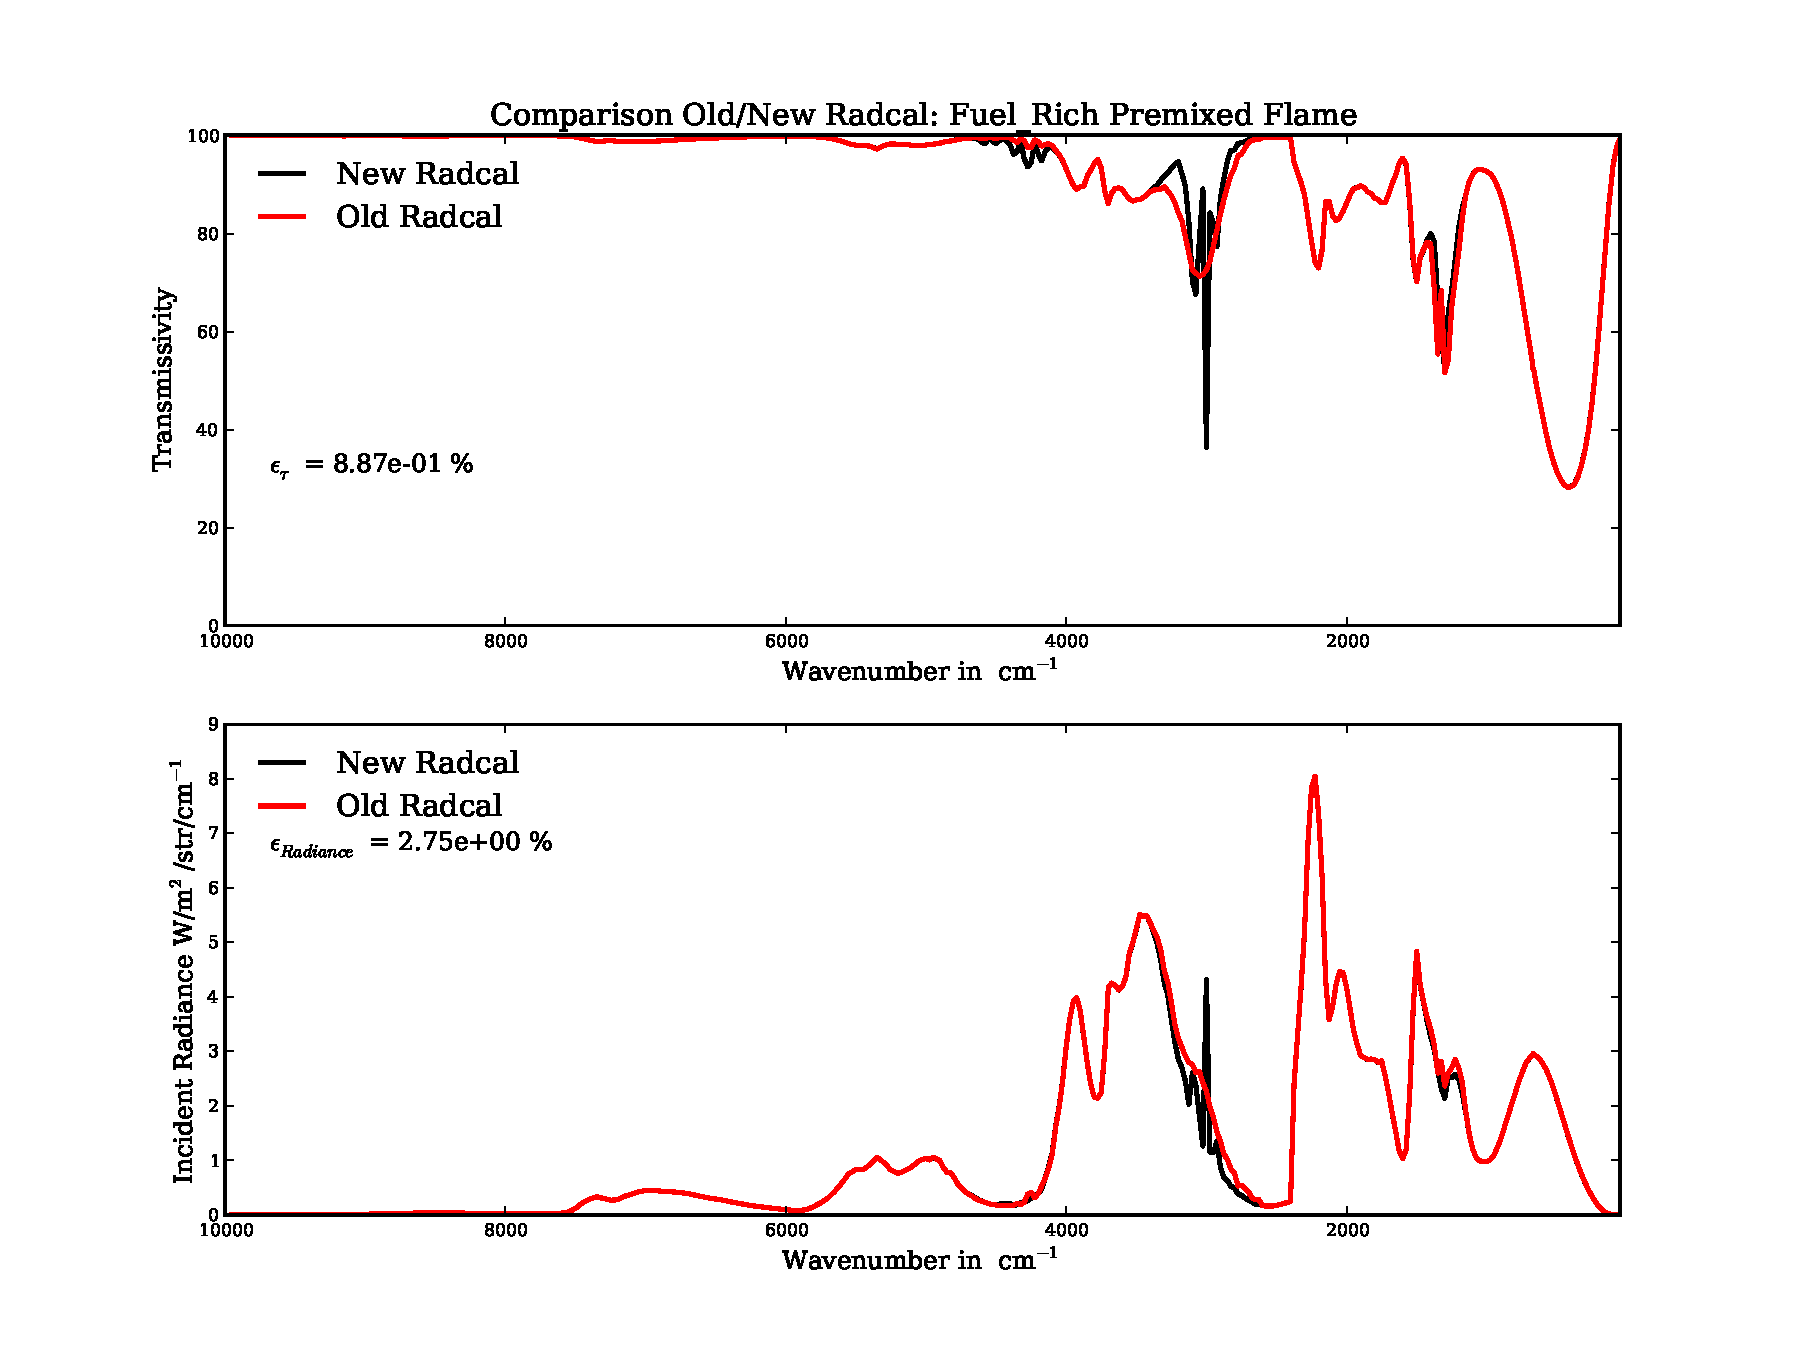
\includegraphics[width=\textwidth]{Figures/Comp_old_new_Premixed_Flame_newCH4.pdf}
\caption{Top: spectral transmissivity, $\bar{\tau}(\om_0; \infty \rightarrow 0)$ (the observer is in $0$, in \%, for a simulated 20~mm thick fuel rich premixed methane/$\rm N_2$/$\rm O_2$ flame at 606~kPa. Red line: predicted results using the previous version of RadCal. Black line: predicted results using the new version of RadCal. Bottom: predicted incident spectral intensity, $I_{\om_0}(0)$, given in $\rm W/m^{2}/str/cm^{-1}$ .\label{fig:Test6_Premixed}}
\end{figure}


\section{Test 7: methanol pool fire}

In this section, predicted results for a 30~cm methanol pool fire are presented in this section. Measurements were made by Aykut Yilmaz, see Ref.~\cite{Yilmaz2008}. Temperature data were averaged over three different tests using the same configuration. Species mole fraction were obtained by gas chromatography. Table~\ref{table::test7_methanol} tabulates the experimental values used for this simulation.
\begin{table}[ht]
\centering
\caption{Measured temperature and species mole fraction as function of the height above the pool surface for a 30~cm diameter methanol pool fire. Data were obtained from Yilmaz, see Ref.~\cite{Yilmaz2008}.\label{table::test7_methanol}}
    \tiny
\begin{tabular}{llllllllllll}
\hline
X(cm) & Temp (K) & XH2 & XO2 & XN2 & XCH4 & XCO & XCO2 & XC2H4 & XC2H2 & XH2O & XCH3OH\\
\hline
55 & 1101.2 & 5.91E-5 & 1.78E-1 & 7.61E-1 & 0.00E+0 & 0.00E+0 & 1.29E-2 & 0.00E+0 & 0.00E+0 & 7.62E-2 & 0.00E+0\\
40 & 1257.7 & 1.99E-3 & 1.54E-1 & 7.42E-1 & 0.00E+0 & 2.90E-3 & 2.18E-2 & 0.00E+0 & 0.00E+0 & 1.01E-1 & 3.27E-4\\
37.5 & 1267.1 & 2.97E-3 & 1.48E-1 & 7.36E-1 & 0.00E+0 & 4.20E-3 & 2.41E-2 & 0.00E+0 & 0.00E+0 & 1.12E-1 & 5.93E-4\\
30 & 1295 & 7.79E-3 & 1.25E-1 & 7.11E-1 & 0.00E+0 & 1.06E-2 & 3.10E-2 & 0.00E+0 & 0.00E+0 & 1.39E-1 & 2.64E-3\\
27.5 & 1284.4 & 5.62E-3 & 1.36E-1 & 7.19E-1 & 0.00E+0 & 6.94E-3 & 2.59E-2 & 0.00E+0 & 0.00E+0 & 1.35E-1 & 1.73E-3\\
20 & 1013.7 & 2.45E-2 & 8.35E-2 & 6.54E-1 & 0.00E+0 & 2.89E-2 & 3.98E-2 & 9.24E-6 & 3.05E-5 & 1.91E-1 & 1.25E-2\\
17.5 & 968.4 & 3.33E-2 & 7.96E-2 & 6.35E-1 & 0.00E+0 & 3.51E-2 & 3.75E-2 & 2.29E-5 & 3.07E-5 & 1.91E-1 & 1.81E-2\\
10 & 820.9 & 4.25E-2 & 5.80E-2 & 5.96E-1 & 4.43E-4 & 4.54E-2 & 4.11E-2 & 3.93E-5 & 7.17E-5 & 2.26E-1 & 4.87E-2\\
7.5 & 768.4 & 4.45E-2 & 5.24E-2 & 5.83E-1 & 5.31E-4 & 4.82E-2 & 4.17E-2 & 4.45E-5 & 8.31E-5 & 2.34E-1 & 6.36E-2\\
5 & 716 & 6.09E-2 & 3.39E-2 & 5.16E-1 & 1.16E-3 & 5.96E-2 & 3.92E-2 & 5.94E-5 & 1.05E-4 & 2.39E-1 & 1.44E-1\\
2.5 & 663.5 & 7.03E-2 & 1.93E-2 & 3.94E-1 & 1.38E-3 & 6.37E-2 & 3.25E-2 & 7.21E-5 & 1.29E-4 & 2.15E-1 & 3.72E-1\\
1.5 & 642.5 & 6.55E-2 & 1.18E-2 & 3.28E-1 & 1.27E-3 & 5.63E-2 & 3.00E-2 & 7.91E-5 & 1.30E-4 & 1.97E-1 & 5.57E-1\\
\hline
\end{tabular}
 \end{table}


The RadCal input file is presented below:

 \begin{lstlisting}
 &HEADER TITLE = "Methanol_Pool_Fire_30cm" CHID = "Methanol_Pool_Fire_30cm"/

&BAND OMMIN = 50.0
      OMMAX = 10000.0/

&WALL TWALL = 300.0 /
&Path_Segment ! Define a homogeneous segment
	T		= 642.5	! Temperature in Kelvin
	LENGTH		= 5.0000000000E-03	! Length of the segment in meters
	PRESSURE	= 1		! Pressure in atm
	XO2		= 1.1819200000E-02	! Mole fraction of O2
	XH2O		= 1.9712830000E-01	! Mole fraction of H2O
	XCO		= 5.6268490000E-02	! Mole fraction of CO
	XCO2		= 3.0011090000E-02	! Mole fraction of CO2
	XC2H4		= 7.9050000000E-05	! Mole fraction of C2H4
	XCH4		= 1.2657700000E-03	! Mole fraction of CH4
	XC2H6		= 0.0000000000E+00	! Mole fraction of C2H6
	XCH3OH		= 5.5659982000E-01	! Mole fraction of CH3OH
	XN2		= 1.4682828000E-01/	! Mole fraction of N2

&Path_Segment ! Define a homogeneous segment
	T		= 663.5	! Temperature in Kelvin
	LENGTH		= 1.7500000000E-02	! Length of the segment in meters
	PRESSURE	= 1		! Pressure in atm
	XO2		= 1.9288640000E-02	! Mole fraction of O2
	XH2O		= 2.1510620000E-01	! Mole fraction of H2O
	XCO		= 6.3724220000E-02	! Mole fraction of CO
	XCO2		= 3.2544630000E-02	! Mole fraction of CO2
	XC2H4		= 7.2090000000E-05	! Mole fraction of C2H4
	XCH4		= 1.3836300000E-03	! Mole fraction of CH4
	XC2H6		= 0.0000000000E+00	! Mole fraction of C2H6
	XCH3OH		= 3.7249435000E-01	! Mole fraction of CH3OH
	XN2		= 2.9538624000E-01/	! Mole fraction of N2

&Path_Segment ! Define a homogeneous segment
	T		= 716	! Temperature in Kelvin
	LENGTH		= 2.5000000000E-02	! Length of the segment in meters
	PRESSURE	= 1		! Pressure in atm
	XO2		= 3.3932530000E-02	! Mole fraction of O2
	XH2O		= 2.3930719000E-01	! Mole fraction of H2O
	XCO		= 5.9551970000E-02	! Mole fraction of CO
	XCO2		= 3.9167250000E-02	! Mole fraction of CO2
	XC2H4		= 5.9430000000E-05	! Mole fraction of C2H4
	XCH4		= 1.1647400000E-03	! Mole fraction of CH4
	XC2H6		= 0.0000000000E+00	! Mole fraction of C2H6
	XCH3OH		= 1.4355283000E-01	! Mole fraction of CH3OH
	XN2		= 4.8326406000E-01/	! Mole fraction of N2

&Path_Segment ! Define a homogeneous segment
	T		= 768.4	! Temperature in Kelvin
	LENGTH		= 2.5000000000E-02	! Length of the segment in meters
	PRESSURE	= 1		! Pressure in atm
	XO2		= 5.2375440000E-02	! Mole fraction of O2
	XH2O		= 2.3403434000E-01	! Mole fraction of H2O
	XCO		= 4.8155710000E-02	! Mole fraction of CO
	XCO2		= 4.1740150000E-02	! Mole fraction of CO2
	XC2H4		= 4.4500000000E-05	! Mole fraction of C2H4
	XCH4		= 5.3133000000E-04	! Mole fraction of CH4
	XC2H6		= 0.0000000000E+00	! Mole fraction of C2H6
	XCH3OH		= 6.3614460000E-02	! Mole fraction of CH3OH
	XN2		= 5.5950407000E-01/	! Mole fraction of N2

&Path_Segment ! Define a homogeneous segment
	T		= 820.9	! Temperature in Kelvin
	LENGTH		= 5.0000000000E-02	! Length of the segment in meters
	PRESSURE	= 1		! Pressure in atm
	XO2		= 5.8036420000E-02	! Mole fraction of O2
	XH2O		= 2.2611716000E-01	! Mole fraction of H2O
	XCO		= 4.5352720000E-02	! Mole fraction of CO
	XCO2		= 4.1128540000E-02	! Mole fraction of CO2
	XC2H4		= 3.9310000000E-05	! Mole fraction of C2H4
	XCH4		= 4.4256000000E-04	! Mole fraction of CH4
	XC2H6		= 0.0000000000E+00	! Mole fraction of C2H6
	XCH3OH		= 4.8728810000E-02	! Mole fraction of CH3OH
	XN2		= 5.8015448000E-01/	! Mole fraction of N2

&Path_Segment ! Define a homogeneous segment
	T		= 968.4	! Temperature in Kelvin
	LENGTH		= 5.0000000000E-02	! Length of the segment in meters
	PRESSURE	= 1		! Pressure in atm
	XO2		= 7.9642260000E-02	! Mole fraction of O2
	XH2O		= 1.9075471000E-01	! Mole fraction of H2O
	XCO		= 3.5088720000E-02	! Mole fraction of CO
	XCO2		= 3.7473970000E-02	! Mole fraction of CO2
	XC2H4		= 2.2860000000E-05	! Mole fraction of C2H4
	XCH4		= 0.0000000000E+00	! Mole fraction of CH4
	XC2H6		= 0.0000000000E+00	! Mole fraction of C2H6
	XCH3OH		= 1.8066990000E-02	! Mole fraction of CH3OH
	XN2		= 6.3895049000E-01/	! Mole fraction of N2

&Path_Segment ! Define a homogeneous segment
	T		= 1013.7	! Temperature in Kelvin
	LENGTH		= 5.0000000000E-02	! Length of the segment in meters
	PRESSURE	= 1		! Pressure in atm
	XO2		= 8.3520100000E-02	! Mole fraction of O2
	XH2O		= 1.9127008000E-01	! Mole fraction of H2O
	XCO		= 2.8887410000E-02	! Mole fraction of CO
	XCO2		= 3.9827410000E-02	! Mole fraction of CO2
	XC2H4		= 9.2300000000E-06	! Mole fraction of C2H4
	XCH4		= 0.0000000000E+00	! Mole fraction of CH4
	XC2H6		= 0.0000000000E+00	! Mole fraction of C2H6
	XCH3OH		= 1.2516090000E-02	! Mole fraction of CH3OH
	XN2		= 6.4396968000E-01/	! Mole fraction of N2

&Path_Segment ! Define a homogeneous segment
	T		= 1284.4	! Temperature in Kelvin
	LENGTH		= 5.0000000000E-02	! Length of the segment in meters
	PRESSURE	= 1		! Pressure in atm
	XO2		= 1.3624232000E-01	! Mole fraction of O2
	XH2O		= 1.3468054000E-01	! Mole fraction of H2O
	XCO		= 6.9395300000E-03	! Mole fraction of CO
	XCO2		= 2.5908820000E-02	! Mole fraction of CO2
	XC2H4		= 0.0000000000E+00	! Mole fraction of C2H4
	XCH4		= 0.0000000000E+00	! Mole fraction of CH4
	XC2H6		= 0.0000000000E+00	! Mole fraction of C2H6
	XCH3OH		= 1.7271700000E-03	! Mole fraction of CH3OH
	XN2		= 6.9450162000E-01/	! Mole fraction of N2

&Path_Segment ! Define a homogeneous segment
	T		= 1295	! Temperature in Kelvin
	LENGTH		= 5.0000000000E-02	! Length of the segment in meters
	PRESSURE	= 1		! Pressure in atm
	XO2		= 1.2502657000E-01	! Mole fraction of O2
	XH2O		= 1.3947277000E-01	! Mole fraction of H2O
	XCO		= 1.0584120000E-02	! Mole fraction of CO
	XCO2		= 3.0954850000E-02	! Mole fraction of CO2
	XC2H4		= 0.0000000000E+00	! Mole fraction of C2H4
	XCH4		= 0.0000000000E+00	! Mole fraction of CH4
	XC2H6		= 0.0000000000E+00	! Mole fraction of C2H6
	XCH3OH		= 2.6410300000E-03	! Mole fraction of CH3OH
	XN2		= 6.9132066000E-01/	! Mole fraction of N2

&Path_Segment ! Define a homogeneous segment
	T		= 1267.1	! Temperature in Kelvin
	LENGTH		= 5.0000000000E-02	! Length of the segment in meters
	PRESSURE	= 1		! Pressure in atm
	XO2		= 1.4815693000E-01	! Mole fraction of O2
	XH2O		= 1.1201391000E-01	! Mole fraction of H2O
	XCO		= 4.1990100000E-03	! Mole fraction of CO
	XCO2		= 2.4057230000E-02	! Mole fraction of CO2
	XC2H4		= 0.0000000000E+00	! Mole fraction of C2H4
	XCH4		= 0.0000000000E+00	! Mole fraction of CH4
	XC2H6		= 0.0000000000E+00	! Mole fraction of C2H6
	XCH3OH		= 5.9345000000E-04	! Mole fraction of CH3OH
	XN2		= 7.1097947000E-01/	! Mole fraction of N2

&Path_Segment ! Define a homogeneous segment
	T		= 1257.7	! Temperature in Kelvin
	LENGTH		= 8.7500000000E-02	! Length of the segment in meters
	PRESSURE	= 1		! Pressure in atm
	XO2		= 1.5356568000E-01	! Mole fraction of O2
	XH2O		= 1.0119799000E-01	! Mole fraction of H2O
	XCO		= 2.8958400000E-03	! Mole fraction of CO
	XCO2		= 2.1753130000E-02	! Mole fraction of CO2
	XC2H4		= 0.0000000000E+00	! Mole fraction of C2H4
	XCH4		= 0.0000000000E+00	! Mole fraction of CH4
	XC2H6		= 0.0000000000E+00	! Mole fraction of C2H6
	XCH3OH		= 3.2715000000E-04	! Mole fraction of CH3OH
	XN2		= 7.2026021000E-01/	! Mole fraction of N2

&Path_Segment ! Define a homogeneous segment
	T		= 1101.2	! Temperature in Kelvin
	LENGTH		= 7.5000000000E-02	! Length of the segment in meters
	PRESSURE	= 1		! Pressure in atm
	XO2		= 1.7842988000E-01	! Mole fraction of O2
	XH2O		= 7.6186860000E-02	! Mole fraction of H2O
	XCO		= 0.0000000000E+00	! Mole fraction of CO
	XCO2		= 1.2909800000E-02	! Mole fraction of CO2
	XC2H4		= 0.0000000000E+00	! Mole fraction of C2H4
	XCH4		= 0.0000000000E+00	! Mole fraction of CH4
	XC2H6		= 0.0000000000E+00	! Mole fraction of C2H6
	XCH3OH		= 0.0000000000E+00	! Mole fraction of CH3OH
	XN2		= 7.3247346000E-01/	! Mole fraction of N2
 \end{lstlisting}


\begin{figure}
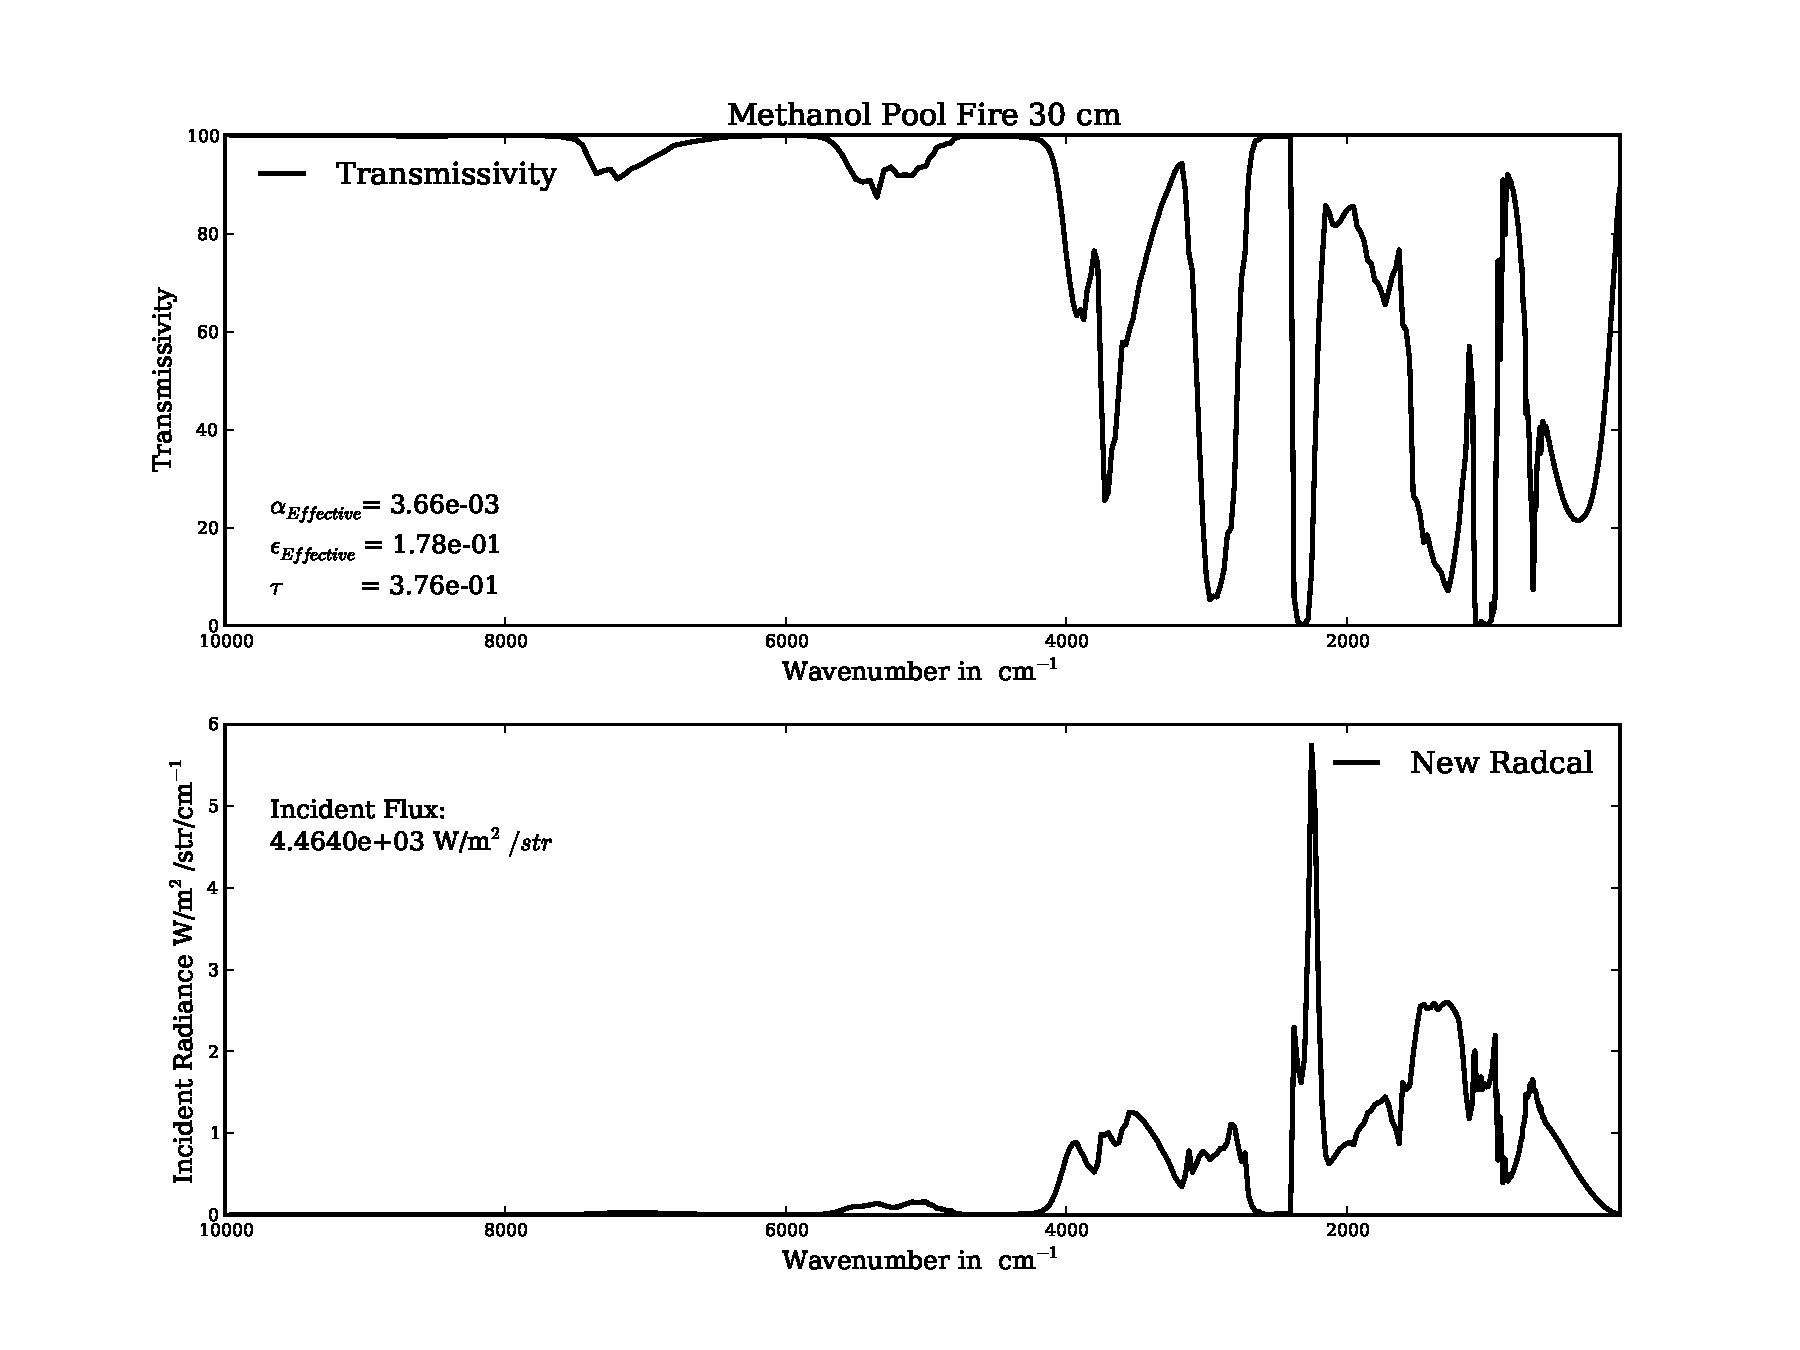
\includegraphics[width=\textwidth]{Figures/Methanol_Pool_Fire_30cm.pdf}
\caption{Top: Predicted spectral transmissivity for a 30~cm diameter methanol pool fire. The measured temperature and species mole fractions are tabulated in Table~\ref{table::test7_methanol}. Bottom: Predicted spectral incident radiative intensity to the surface of the pool fire. Emission by $\rm CO_2$ is responsible for the main spike located between 2100--2500~$\rm cm^{-1}$.\label{fig:Test7_Methanol}}
\end{figure}

